\subsection{Zadanie 1 -- Najmniejszy zbiór dominujący}
\paragraph{Treść:}
\textit{Zbiór dominujący} w grafie $G$ to podzbiór wierzchołków 
$D \subset V(G)$ taki, że każdy wierzchołek grafu $G$
należy do $D$ lub ma przynajmniej jednego sąsiada w $D$.

Zaprojektuj jak najwydajniejszy algorytm, który znajdzie rozmiar najmniejszego zbioru dominującego w zadanym
grafie o $n$ wierzchołkach i maksymalnym stopniu nie większym niż 3. Oszacuj złożoność tego algorytmu.

\paragraph{Rozwiązanie:}
Aby rozwiązać to zadanie zastosujemy algorytm z nawrotami.

Wprowadźmy oznaczenia, które zostaną wykorzystane w algorytmie.
Niech $D_{\min}$ to najmniejszy zbiór dominujący jaki udało 
nam się dotychczas znaleźć.
Niech $D$ to aktualny stan zbioru dominującego, oraz
niech $X$ to zbiór wierzchołków, które na pewno nie znajdą się 
w zbiorze dominującym $D$ na następnych poziomach rekurencji.
Warunkiem stopu będzie sytuacja, w której $|D| + |X| = |V(G)|$.

Możemy wprowadzić optymalizację polegająca na tym, że 
przestaniemy badać daną gałąź wykonań rekurencyjnych,
w przypadku, kiedy $|D| < |D_{\min}|$. Optymalizacji tej nie będziemy
stosowali w przypadku kiedy $D_{\min}$ nie zostało jeszcze znalezione,
w tym celu skorzystamy z faktu, że jeśli graf $G$, jest 
taki, że $V(G) \not = \emptyset$,
to każdy zbiór dominujący dla tego grafu nie jest pusty.

W poniższym algorytmie, przyjmujemy, że $D_{\min}$ to globalny zbiór
wierzchołków, który początkowo jest pusty.
\begin{algorithm}[H]
	\caption{Algorytm znajdowania najmniejszego zbioru dominującego}
	\begin{algorithmic}[1]
		\Procedure{DominatingSet}{$G$: graf, $D$: zbiór, $X$: zbiór}
		\If{$|D| > |D_{min}| \land |D_{min}| \not = \emptyset$}
		\State \Return
		\EndIf
		\State Niech $Y$ to zbiór wierzchołków niezdominowanych, tzn. takich, które nie mają żadnego sąsiada w zbiorze $D$ (żaden
		wierzchołek z $Y$ nie należy do $X$ ani $D$)		

		\If{$Y = \emptyset$}
		\If{Każdy wierzchołek z $X$ jest zdominowany}
		\State $D_{\min} = D$
		\EndIf
		\State \Return
		\EndIf
		\State Niech $u$ to dowolny wierzchołek z $Y$
		\State DominatingSet($G$, $D \cup \{u\}$, $X$, $D_{\min}$)
		\If{$|N(u)| \geq 1$}
		\State Niech $v_1 \in N(X)$
		\If{$v_1 \not \in D \land v_1 \not \in X$}
		\State DominatingSet($G$, $D \cup \{v_1\}$, $X \cup \{u\}$, $D_{\min}$)
		\EndIf
		\EndIf
		\If{$|N(u)| \geq 2$}
		\State Niech $v_2 \in N(X) \setminus \{v_1\}$
		\If{$v_2 \not \in D \land v_2 \not \in X$}
		\State DominatingSet($G$, $D \cup \{v_2\}$, $X \cup \{u, v_1\}$, $D_{\min}$)
		\EndIf
		\EndIf
		\If{$|N(u)| = 3$}
		\State Niech $v_3 \in N(X) \setminus \{v_1, v_2\}$
		\If{$v_3 \not \in D \land v_3 \not \in X$}
		\State DominatingSet($G$, $D \cup \{v_3\}$, $X \cup \{u, v_1, v_2\}$, $D_{\min}$)
		\EndIf
		\EndIf
		\EndProcedure		
	\end{algorithmic}
\end{algorithm}

Aby oszacować złożoność powyższego algorytmu skorzystamy z 
twierdzenia o rozwiązywaniu rekurencji. Przez $f(n)$
oznaczmy pesymistyczny czas działania funkcji \textsc{DominatingSet},
wtedy prawdą jest, że
\[f(n) \leq f(n-1) + f(n-1) + f(n-2) + f(n-3) + f(n-4) + O(n),\]
gdzie $O(n)$ to złożoność znajdowania zbioru $Y$. 
Szukamy pierwiastka poniższego równania
\[x^4 = x^3 + x^2 + x + 1,\]
po rozwiązaniu powyższego równania, otrzymamy największy
pierwiastek $x \approx 1.9276$. Zatem na mocy twierdzenia
o rozwiązywaniu rekurencji złożoność algorytmu wynosi $O(n1.9276^n) = O^*(1.9276^n)$.

\subsection{Zadanie 3 -- Kolorowanie grafu z list o rozmiarze nie większym niż 2}
\paragraph{Treść:} W problemie kolorowania grafu $G$ z list dla każdego wierzchołka 
$v \in V(G)$ mamy daną listę $L_v$ i
szukamy poprawnego kolorowania grafu $G$, w którym kolor każdego wierzchołka $v$ należy do $L_v$.
Zaprojektuj algorytm, który rozwiąże problem kolorowania grafu z list w czasie wielomianowym w przypadku, gdy
wszystkie listy mają rozmiar nie większy niż $2$.

\paragraph{Rozwiązanie:} 

Niech graf $G$ będzie grafem wejściowym takim, że

$V(G) = \{v_1, v_2, \ldots, v_n\}$. 
Utwórzmy zbiór wierzchołków
\[V' = \{v_{ik} : v_i\in V(G) \land k \in L_{v_i}\}\]

oraz zbiór krawędzi 
\[E' = \underbrace{\{v_{ik}v_{il} : v_i \in V(G) \land k, l \in L_{v_i}\}}_\text{krawędzie list} \cup 
\underbrace{\{v_{ik}v_{jk} : v_iv_j \in E(G) \land k\in L_{v_i} \cap L_{v_j}\}}_\text{krawędzie kolorów}.\]

Niech graf $G' = (V', E')$. 

Oznacza to, że każdy wierzchołek z $V(G)$ rozbijamy na dwa wierzchołki w $V'$ odpowiadające kolorom z listy (lub jeden, jeśli na liście znajduje się tylko jeden kolor) i tworzymy pomiędzy 
nimi krawędź. Pozostałe krawędzie pomiędzy dwoma wierzchołkami
$u$ i $v$ z $G'$ tworzymy wtedy, kiedy wierzchołki,
z których $u$ i $v$ zostały rozbite, sąsiadują ze sobą
w grafie $G$ oraz $u$ i $v$ odpowiadają temu samemu kolorowi (rysunek \ref{fig:kolorowanielistowe}). 

Teraz zauważmy, że graf $G'$ jest dwudzielny oraz każdy wierzchołek z $G$ ma swojego odpowiednika w \emph{tej samej} klasie dwudzielności $X$ wtedy i tylko wtedy, gdy możemy pokolorować $G$ listowo. 

\begin{figure}[H]
\centering
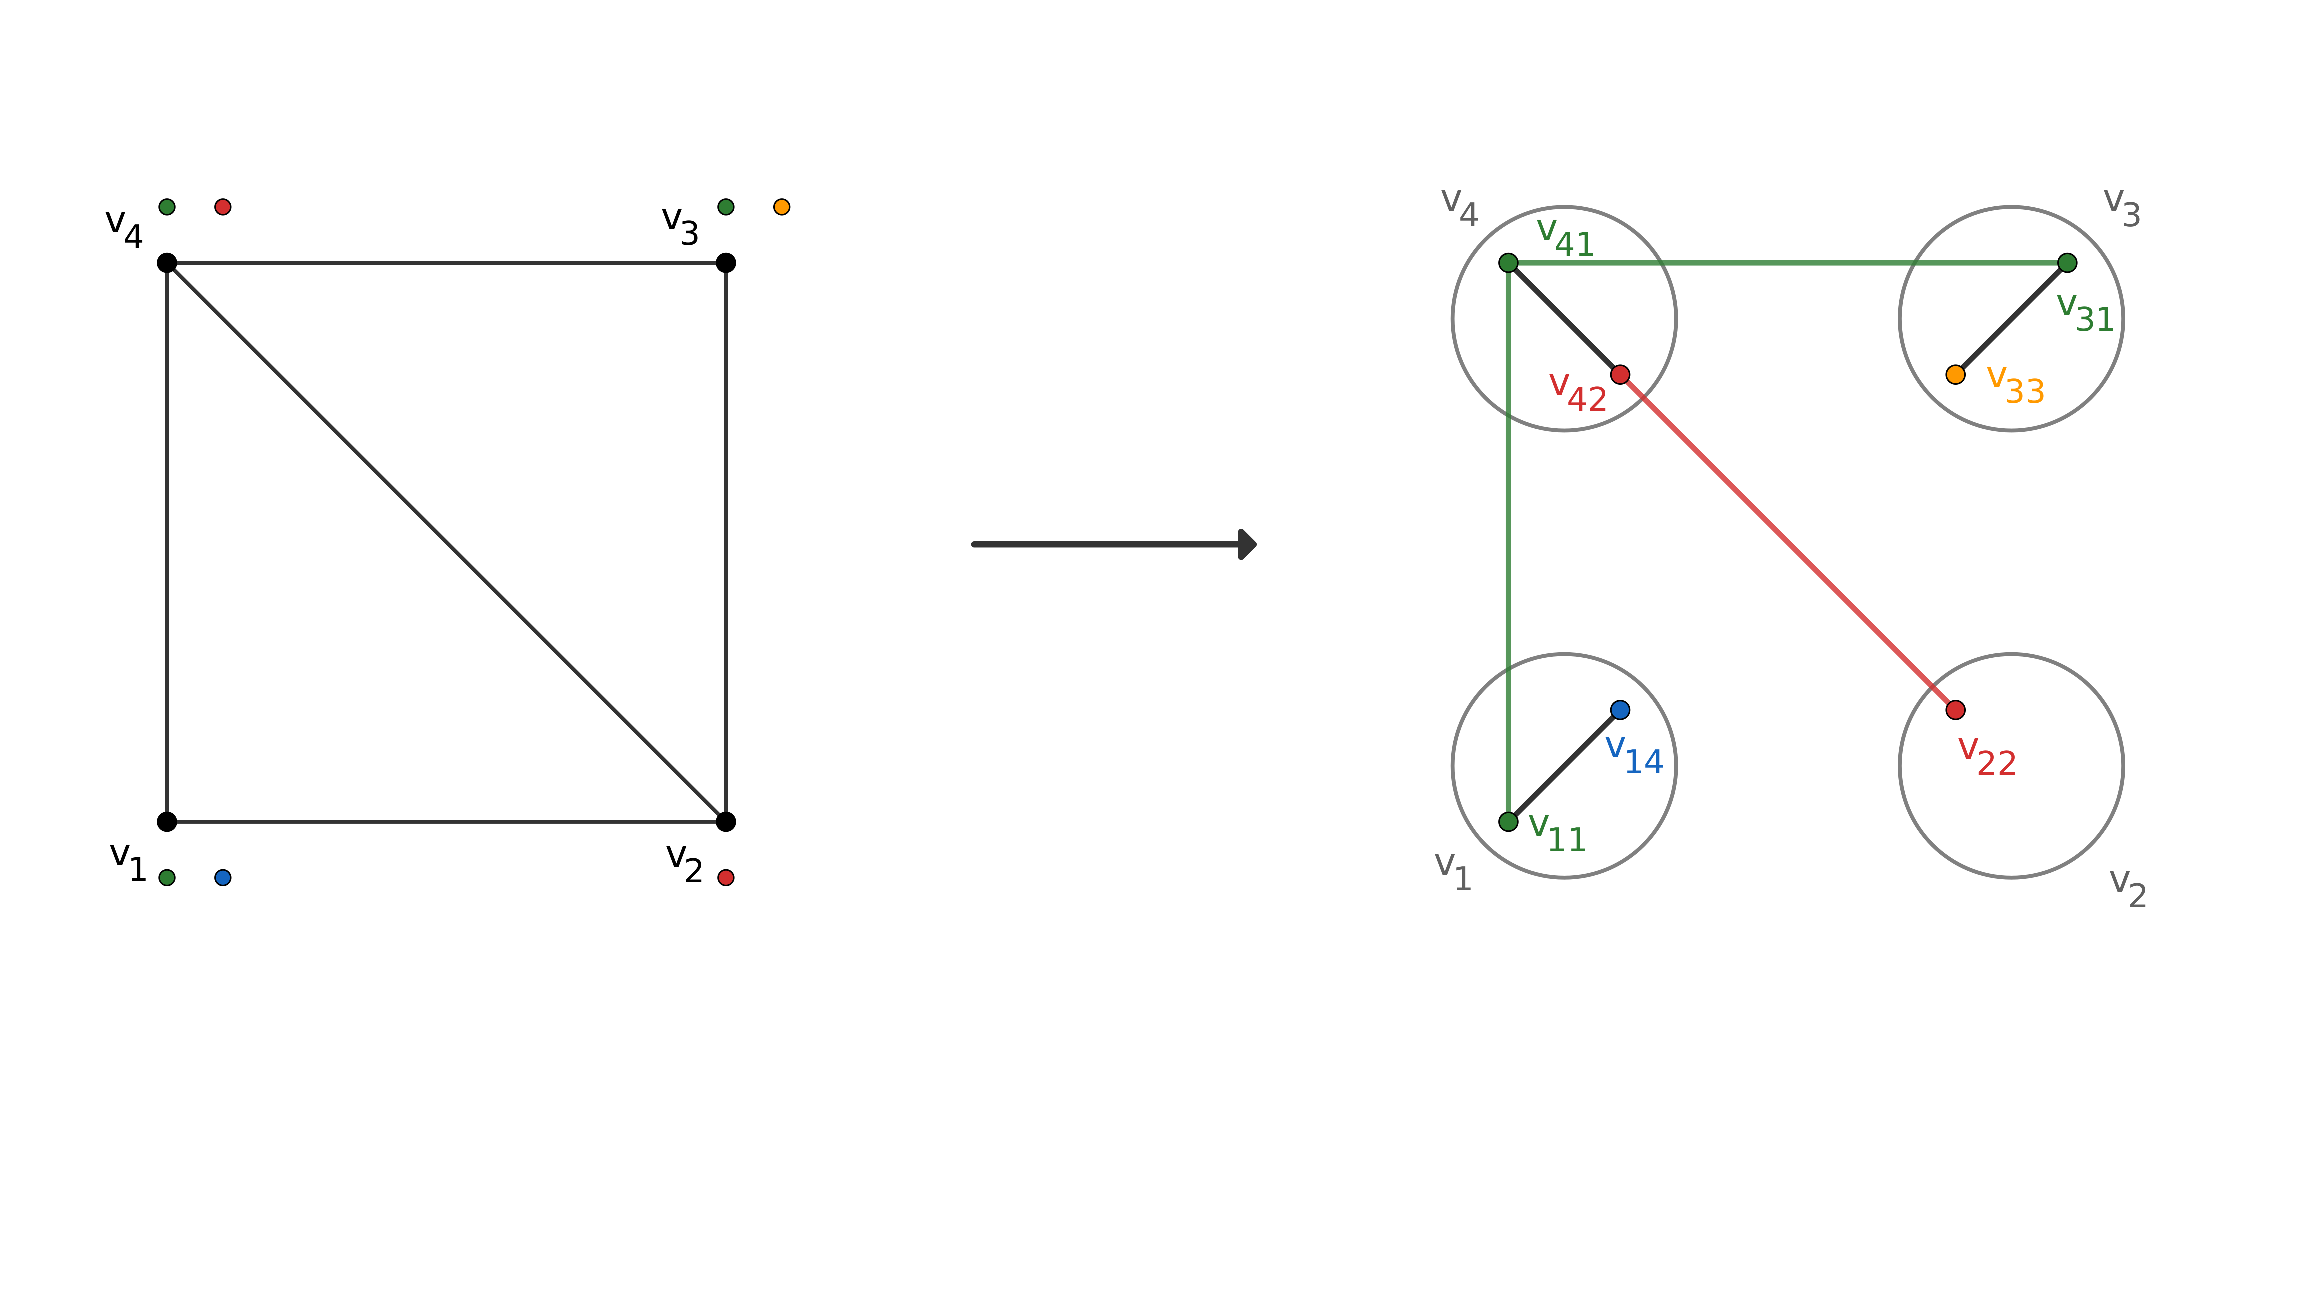
\includegraphics[trim=0 150 0 60,clip,width=\linewidth]{data/3listcol.eps}
\caption{Przykładowy przebieg konstrukcji nowego grafu. Można zauważyć, że powstały graf jest dwudzielny, a $v_{14}$, $v_{22}$, $v_{33}$ i $v_{41}$ tworzą żądaną klasę dwudzielności $X$, zatem oryginalny graf da się pokolorować listowo.}
\label:{fig:kolorowanielistowe}
\end{figure}

Dzieje się tak dlatego, że dla każdego wierzchołka $v_i\in V(G)$ klasa $X$ zawiera wierzchołek $v_{ik}$ reprezentujący pokolorowanie $v_i$ na kolor $k$. Zawiera ona dokładnie jeden wierzchołek $v_{ik}$ odpowiadający $v_i$ ze względu na obecność krawędzi łączących $v_{ik}$ z $v_{il}$ dla $l \in L_{v_i}, l \neq k$ (tzn. z innymi kolorami z $L_{v_i}$). Jednocześnie z dwudzielności wynika, że dla każdego koloru $k$ w klasie $X$ nie sąsiadują żadne wierzchołki $v_{ik}$, $v_{jk}$ takie, że $v_iv_j\in E(G)$. Kolorowanie to jest więc poprawne.

Pokazanie, że jeżeli istnieje poprawne kolorowanie listowe grafu $G$, to $G'$ jest dwudzielny i odpowiednie wierzchołki $G'$ odpowiadające temu kolorowaniu tworzą klasę dwudzielności jest analogiczne. 

Pozostaje pytanie, jak można zaimplementować powyższe rozumowanie. Jeżeli $G'$ jest dwudzielnym grafem spójnym to istnieje dokładnie jeden podział na klasy dwudzielności. W takiej sytuacji możemy znaleźć klasy dwudzielności oraz zbadać, czy wszystkie wierzchołki z $G$ mają swojego odpowiednika w tej samej klasie. W przypadku kiedy $G'$ nie jest spójny, możemy w sposób analogiczny rozważyć jego spójne składowe. Problem dwudzielności jak i znajdowania składowych grafu potrafimy rozwiązać (patrz \hyperref[exc:bipart]{zadania 4 oraz 5 z tematu ,,Przeszukiwanie grafów''}.

Utworzenie zbiorów, dwudzielność oraz znajdowanie składowych grafu są problemami wymagającymi czasu wielomianowego, a zatem algorytm spełnia wymagania czasowe.

